\documentclass[a4paper, twocolumn, 11pt, twoside]{article}

% update your language here.
\usepackage[brazil]{babel}
\usepackage{linguamatica}

% This assumes your files are encoded as UTF8
\usepackage[utf8]{inputenc}
\usepackage{amssymb} % For symbols like ? in glosses


\usepackage[T1]{fontenc}
\usepackage{xcolor}   % For color
\usepackage{graphicx} % For handling images (optional)
\usepackage{fancyhdr} % For custom headers/footers (optional)

\definecolor{ForestGreen}{RGB}{34,139,34}
\definecolor{Maroon}{RGB}{128,0,0}

\definecolor{lightgray}{RGB}{224, 224, 224}
\definecolor{mblue}{RGB}{0, 127, 204}
\definecolor{lightyellow}{RGB}{255, 247, 209}
\definecolor{lightblue}{RGB}{204, 230, 255} % 

%% Please use UTF8 in your document

%% Set the bibliography style.
%% Styles provided for Spanish (Castilian), Catalan and Portuguese.
%% Other languages will be created on a required basis.

\bibliographystyle{sp_por}   % This for Portuguese

%% You can leave this unchanged. It will be updated by the editors when your paper gets published.
\submitted{15 de \OCT{} 2017}
\accepted{3 de \DEC{} 2017}

%% Add your title in the main language used in the article
\title{Desafios na Tradução da Informação Espacial do EN para o PT-br}

%% Currenty the title in English is also mandatory
\titleEN{Challenges in Translating Spatial Information from EN to PT-br}


%% Add authors here. Three lines for each author.
%% First line with author name, second with the affiliation and third with e-mail
%% In cases where a second line is needed for the affiliation, use the command \nl to separate them. 
\author{
  Rafael Fernandes
  \instituto{Universidade de São Paulo}
  \email{rafael.macario@usp.br} 
  \and 
  Rodrigo Souza
 \instituto{Universidade de São Paulo}
  \email{rodrigo.aparecido.souza@usp.br}
  \and
  Marcos Lopes
  \instituto{Universidade de São Paulo}
  \email{marcoslopes@usp.br}
  \and
%%  Paulo Santos
%%  \instituto{Flinders University}
%%  \email{paulo.santos@flinder.edu.au}
%%%%  \and
%%  Thomas Finbow
%%  \instituto{Universidade de São Paulo}
%%  \email{thomas.finbow@usp.br}
}


\begin{document}
\maketitle

%% Add the abstract in the main language for the article. If possible, doesn't add any citations here.
\begin{resumo}
  A Tradução Automática Neural (TAN), apesar de ser a abordagem dominante, ainda enfrenta desafios significativos ao traduzir conhecimento espacial. Neste estudo, utilizamos o Raciocínio Espacial Qualitativo (REQ) para representar e analisar informações espaciais em traduções automáticas do inglês para o português. Foram traduzidas 145 frases dos corpora CAM e COCA, utilizando os sistemas Google Translate e DeepL. Ao mapear logicamente as diferenças de significado entre as traduções e os originais, utilizando o REQ, identificamos que a TAN comete em média 10,6\% de erros semânticos e 12\% de erros de projeção sintática em traduções envolvendo conceitos espaciais. Nossos resultados evidenciam a necessidade de aprimorar os modelos de TAN para lidar com as nuances da linguagem espacial, contribuindo para o avanço da pesquisa em tradução automática.
\end{resumo}

%% Add keywords in the article main language, in lowercase
\palavraschave{tradução automática neural; semântica espacial; raciocínio espacial qualitativo; tradução automática inglês-português; polissemia; tipologia linguística}

%% Add the abstract in English
\begin{abstract}
  Neural Machine Translation (NMT), currently the leading approach, still faces challenges in translating spatial knowledge. In this study, we used Qualitative Spatial Reasoning (QSR) to represent spatial information in automatic translations from English to Portuguese. We translated $145$ sentences from the CAM and COCA corpora using Google Translate and DeepL, and identified the causes of unnatural translations. Using QSR, we logically mapped the differences in meaning. Our results indicate that, despite generally good performance, NMT struggles with specific spatial meanings, resulting in $10.6\%$ semantic errors and $12.0\%$ syntactic projection errors. This work explores the practical and theoretical challenges of machine translation.
\end{abstract}

%% add the keywords in English
\keywords{neural machine translation; spatial semantics; qualitative spatial reasoning; english-portuguese machine translation; polysemy; language typology}


\section{Introdução}

A Tradução Automática Neural (TAN) tornou-se o paradigma dominante na área de Tradução Automática, tanto em estudos acadêmicos quanto em aplicações práticas \citep{dabre2020survey}. Esse avanço se deve, principalmente, à capacidade aprimorada dos modelos de aprendizado profundo em capturar dependências de longo alcance nas frases \citep{vaswani2017attention, yang2020survey}.

No entanto, apesar dos avanços, alguns tradutores automáticos ainda enfrentam desafios ao lidar com as nuances da linguagem espacial, como a polissemia das preposições e a projeção idiossincrática da maneira de movimento em inglês diretamente para verbos em português \citep{McCleary-Viotti-2004}. Um exemplo disso pode ser visto no Exemplo (1), retirado do Cambridge Online Dictionary (CAM), onde a tradução do inglês (EN) para o português (PT) foi realizada com o Google Translate (GT) e o DeepL (DL).

\footnotesize
  \ex. He swam \emph{across} the river. (CAM)\label{ex:across2}
  \ag. ?~Ele nadou do outro lado do rio. (GT) \\  
  3SG.M swam from-the other side of-the river\\ 
  \bg. Ele atravessou o rio a nado. (DL) \\ 
  3SG.M crossed the river by swimming\\
  \par
\normalsize
  
A tradução do Exemplo~\ref{ex:across2} feita pelo modelo GT, embora gramaticalmente correta, erra ao não capturar a expressão mais natural em PT para a sentença em EN. O DL, por outro lado, acerta.
  
A razão por trás dessa tradução errada está na polissemia da preposição ACROSS, que pode significar tanto uma localização oposta, fixa ao ponto de referência quanto movimento de um lado de um espaço para o outro. Neste caso em particular, o significado pretendido é claramente o último. Para ilustrar isso, vamos considerar as Figuras 1 e 2.

\begin{figure}[ht]
  \centering
  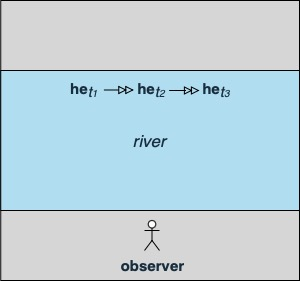
\includegraphics[width=0.3\textwidth]{aa-a-2.jpg}
  \caption{Diagrama semântico de (1)-a.}\label{fig:across-1a}
\end{figure}

\begin{figure}[ht]
  \centering
  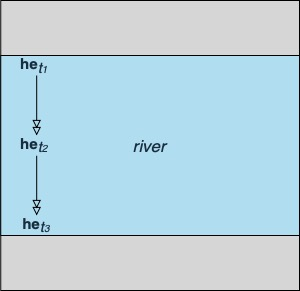
\includegraphics[width=0.3\textwidth]{bb-b-2.jpg}
  \caption{Diagrama semântico de (1)-b.}\label{fig:across-1b}
\end{figure}


A Figura~\ref{fig:across-1a} representa o GT, que indica movimento dentro de um local específico (uma margem oposta do rio). No entanto, a Figura~\ref{fig:across-1b}, representando a saída DL, transmite o significado de cruzar de uma margem do rio para a outra, capturando assim a natureza dinâmica implícita na frase original EN. 

Com isso em mente, este artigo explora a tradução automática de frases em EN que envolvem informações espaciais (topologia ou movimento) para PT, utilizando GT e DL. Nosso objetivo é duplo: primeiro, baseados nos trabalhos de Spranger et al. (2016), Freksa e Kreutzmann (2016) e Randell et al. (1992), formalizamos amostras de frases nas línguas de origem e destino. Em seguida, categorizamos as traduções para identificar erros comuns cometidos por ferramentas de TAN. Em vez de focar no processo de TAN em si, discutiremos os significados espaciais que essas ferramentas têm dificuldade em capturar, iluminando práticas e direções teóricas para pesquisa em linguagem espacial e TA. Nossos resultados mostram que, apesar do bom desempenho geral, os motores de TA ainda cometem erros sistemáticos em algumas categorias ao traduzir textos de EN para PT.


\subsection{Desafios na Tradução da Espacialidade}


\begin{table}[htb]
  \centering
  \begin{tabular}{lrr}
    \toprule
    & \textbf{Homens} & \textbf{Mulheres} \\
    \midrule
    Crianças & 10~032 & 32~341 \\
    Adultos & 23~431 & 9~443 \\
    \bottomrule
  \end{tabular}
  \caption{Exemplo de tabela com poucos traços.}
  \label{tab:1}
\end{table}

\section{Metodologia}
Nesta seção, apresentamos as etapas metodológicas do nosso trabalho, composta pela coleta dos dados, pela classificação das preposições, pelo processo de tradução, pelas formalizações das informações espaciais e pela categorização das traduções. 

\subsection{Coleta dos Dados}

\subsection{Classificação das Preposições}

\subsection{Tradução das Sentenças}

%\subsection{Formalização das Informações Espaciais}

\subsection{Formalização das Sentenças}

A partir do trabalho de~\citet{spranger2016robust}, definimos cada intervalo de tempo $t$ como um conjunto de pontos e utilizamos o predicado \textit{occurs\_in($\theta$, $t$)} para denotar que um evento $\theta$ ocorre durante um intervalo de tempo $t$.
Com base em~\citet{freksa2016neighborhood}, definimos os eventos $\theta$ por meio do cojunto de treze relações qualitativas espaço-temporais apresentadas na Figura~\ref{fig:13_relations}.

\begin{figure}[ht]
	\centering
	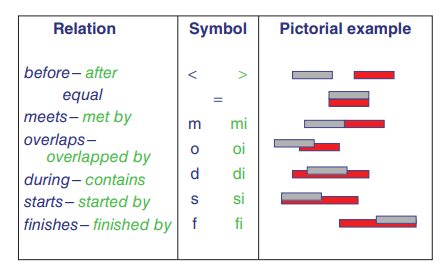
\includegraphics[width=\columnwidth]{Figures/13_concep_neigb_relat.png}
	\caption{Treze relações qualitativas entre dois objectos lineares estendidos sobre uma reta orientada~\citep{freksa2016neighborhood}.}
	\label{fig:13_relations}
\end{figure}

A Figura~\ref{fig:13_relations} apresenta  as treze relações conjuntamente exaustivas e em pares disjuntivos baseadas no Cálculo de Intervalos de Allen~\citep{allen1983maintaining}.
Essas relações podem ser descritas pelo seguinte cojunto: \{\textit{before, after, equal, meets, met by, overlaps, overlapped by, during, contains, starts, started by, finishes, finished by}\}. 
Com esse cojunto de relações, podemos representar transições relacionadas ao movimento de objetos que fazem parte de um evento.

Por \textit{default}, assumimos um espaço 3D para todos os objetos em nossas representações de movimento nas cenas. Para representar as informações espaciais em sentenças como as do Exemplo (1), em que a preposição ``across'' denota
o movimento de atravessar uma superfície, definimos uma função \textit{surface(r)}. Essa função mapeia relações como
\textit{during} ou \textit{contains}, projetando um objeto em uma superfície 2D.

Para modelar relações mereotopológicas, nos baseamos no RCC-8~\citep{randell1992spatial}: \{\textit{dc, ec, po, eq, tpp, ntpp, tpp}${^{-1}}$, \textit{ntpp}${^{-1}}$\}.
Para formalizar uma sentença como a gerada pela tradução do GT no Example~\ref{example:across2}, nós definimos uma Região de Referência (\textit{RR}), que é uma parte de 
uma região \textit{R}, ou Fundo, localizada fora da região onde a ação executada pelo objeto \textit{F}, a Figura, 
acontece. A Região de Referência é separada do restante de \textit{R} por uma linha transversal (chamada por nós de \textit{meridiano}) 
que liga com \textit{R} em dois pontos distantes (não consecutivos) e não toca $F: R_{op} = ntpp(F, R)$.

De modo a representar a relação entre o predicado \textit{occurs\_in($\theta$, $t$)} e as relações qualitativas 
apresentadas na Figura~\ref{fig:13_relations}, nós utilizamos o conectivo $\leftlsquigarrow$, que denota uma implicação
revogável, isto é, uma forma de raciocíno que é racionalmente convincente, mas carece de validade dedutiva. 
Nesse contexto, as premissas do argumento oferecem suporte racional para a conclusão, mas há a possibilidade 
de as premissas serem verdadeiras e a ser falsa. Em resumo, a conexão entre as premissas e a conclusão são provisórias
e podem ser anuladas por informações suplementares.

\subsection{Categorização das Traduções}
%\subsection{title}

\section{Resultados e Discussão}


\begin{table}[!htb]
  \centering
  \scalebox{0.8}{
  \begin{tabular}{| l |p{.3\textwidth}|}%{|l|l|}
  \hline
  \textbf{Original text:} He swam \underline{across} the river. 
  \\\hline\hline
  \begin{tabular}[c]{@{}l@{}}  
  $\forall t$ $ \in \{t_1, t_2, t_3\}, t_1 < t_2 < t_3$\\ 
  $occurs\_in(moves\_across(he, river), t)$ $\leftlsquigarrow$\\
  $river' = surface(river)$ $\wedge$\\
  $starts(he, river', t_1)$ $\wedge$\\ 
  $during(he, river', t_2)$ $\wedge$\\ 
  $finishes(he, river', t_3)$\\
  %$continuous(t_1, t_2, t_3)$\\
  
  \end{tabular}\\\hline\hline
  \textbf{GT:} Ele nadou \underline{do outro lado} do rio. 
  \\\hline\hline
  \begin{tabular}[c]{@{}l@{}}  
  
  $\forall t$ $\in \{t_1, t_2, t_3\}, t_1 < t_2 < t_3$\\
  $occurs\_in(moves\_on\_opposite\_side(he, river_{op}), t)$ $\leftlsquigarrow$\\
  $river' = surface(river_{op})$ $\wedge$\\
  $starts(he, river', t_1)$ $\wedge$\\
  $during(he, river', t_2)$ $\wedge$\\ 
  $finishes(he, river', t_3)$\\
  \end{tabular}\\\hline\hline
  
  \textbf{DL:} Ele \underline{atravessou} o rio a nado.
  \\\hline\hline
  \begin{tabular}[c]{@{}l@{}} 
  $\forall t$ $ \in \{t_1, t_2, t_3\}, t_1 < t_2 < t_3$\\ 
  $occurs\_in(moves\_across(he, river_{op}), t)$ $\leftlsquigarrow$\\
  $river' = surface(river_{op})$ $\wedge$\\
  $starts(he, river', t_1)$ $\wedge$\\ 
  $during(he, river', t_2)$ $\wedge$\\ 
  $finishes(he, river', t_3)$\\
  % $continuous(t_1, t_2, t_3)$\\
  \end{tabular}\\\hline
  
  \end{tabular}}
  \caption{Formalizations for sentences in Example~\ref{example:across2}.}
  \label{table:FormAcross}
  \end{table}


  % Through
\begin{table}[!htb]
  \centering
  \scalebox{0.7}{
  \begin{tabular}{| l |p{.3\textwidth}|}%{|l|l|}
  \hline
  \textbf{Original text:} He struggled \underline{through} the crowd till he\\ reached the front.
  \\\hline\hline
  \begin{tabular}[c]{@{}l@{}}  
  $\forall t$ $\in \{t_1, t_2, t_3\}, t_1 < t_2 < t_3$\\ $occurs\_in(arduously(moves\_through(he, crowd), t))$ $\leftlsquigarrow$\\ 
  $starts(he, crowd, t_1)$ $\wedge$\\  
  $during(he, crowd, t_2)$ $\wedge$\\ 
  $finishes(he, crowd, t_3)$ \\
  \end{tabular}\\\hline\hline
  
  \textbf{GT:} Ele lutou \underline{no meio} da multidão até chegar à frente. 
  \\\hline\hline
  \begin{tabular}[c]{@{}l@{}} 
  $\forall t$ $\in \{t_1, t_2, t_3\}, t_1 < t_2 < t_3$\\
  $occurs\_in(fights(he, crowd)$ $\wedge$ $moves\_to(he, crowd), t)$ $\leftlsquigarrow$\\
  $starts(he, crowd, t_1)$ $\wedge$\\  
  $during(he, crowd, t_2)$ $\wedge$\\ 
  $finishes(he, crowd, t_3)$\\ 
  \end{tabular}\\\hline\hline
  
  \textbf{DL:} Ele se debateu \underline{entre} a multidão até chegar à frente.
  \\\hline\hline
  \begin{tabular}[c]{@{}l@{}} 
  $\forall t$ $\in \{t_1, t_2, t_3\}, t_1 < t_2 < t_3$\\
  $occurs\_in(flounder(he, crowd)$ $\wedge$ $moves\_to(he, crowd), t)$ $\leftlsquigarrow$\\
  $starts(he, crowd, t_1)$ $\wedge$\\  
  $during(he, crowd, t_2)$ $\wedge$\\ 
  $finishes(he, crowd, t_3)$\\  
  \end{tabular}\\\hline
  \end{tabular}}
  \caption{Formalizations for sentences in Example~\ref{example:through1}.}
  \label{table:FormThrough}
  \end{table}



  
  
 
\section{Conclusão}

\section*{Agradecimentos}

Os agradecimentos devem ser colocados sempre numa secção final, sem número, tal como
neste exemplo. Sempre que o autor assim o entender, deverá agradecer aos revisores.


\bibliography{references}


\end{document}
